%%%%%%%%%%%%%%%%%%%%%%%%%%%%%%%%%%%%%%%%%
% Journal Article
% LaTeX Template
% Version 1.3 (9/9/13)
%
% This template has been downloaded from:
% http://www.LaTeXTemplates.com
%
% Original author:
% Frits Wenneker (http://www.howtotex.com)
%
% License:
% CC BY-NC-SA 3.0 (http://creativecommons.org/licenses/by-nc-sa/3.0/)
%
%%%%%%%%%%%%%%%%%%%%%%%%%%%%%%%%%%%%%%%%%

%----------------------------------------------------------------------------------------
%	PACKAGES AND OTHER DOCUMENT CONFIGURATIONS
%----------------------------------------------------------------------------------------

\documentclass[twoside]{article}

\usepackage[utf8]{inputenc} % Permite el uso de acentos directamente
\usepackage[sc]{mathpazo} % Use the Palatino font
\usepackage[T1]{fontenc} % Use 8-bit encoding that has 256 glyphs
\linespread{1.05} % Line spacing - Palatino needs more space between lines
\usepackage{microtype} % Slightly tweak font spacing for aesthetics
\usepackage{adjustbox}
\usepackage{amsmath} % Equations
\usepackage{amssymb} % Equations
\usepackage{color} % Allow colors to be defined
\usepackage{enumerate} % Needed for markdown enumerations to work
\usepackage{fancyvrb} % verbatim replacement that allows latex
\usepackage[hmarginratio=1:1,top=32mm,columnsep=20pt]{geometry} % Document margins
\usepackage{multicol} % Used for the two-column layout of the document
\usepackage[hang, small,labelfont=bf,up,textfont=it,up]{caption} % Custom captions under/above floats in tables or figures
\usepackage{booktabs} % Horizontal rules in tables
\usepackage{float} % Required for tables and figures in the multi-column environment - they need to be placed in specific locations with the [H] (e.g. \begin{table}[H])
\usepackage{hyperref} % For hyperlinks in the PDF

\usepackage{lettrine} % The lettrine is the first enlarged letter at the beginning of the text
\usepackage{paralist} % Used for the compactitem environment which makes bullet points with less space between them

\usepackage{abstract} % Allows abstract customization
\renewcommand{\abstractnamefont}{\normalfont\bfseries} % Set the "Abstract" text to bold
\renewcommand{\abstracttextfont}{\normalfont\small\itshape} % Set the abstract itself to small italic text

\usepackage{titlesec} % Allows customization of titles
\renewcommand\thesection{\Roman{section}} % Roman numerals for the sections
\renewcommand\thesubsection{\Roman{subsection}} % Roman numerals for subsections
\titleformat{\section}[block]{\large\scshape\centering}{\thesection.}{1em}{} % Change the look of the section titles
\titleformat{\subsection}[block]{\large}{\thesubsection.}{1em}{} % Change the look of the section titles

\usepackage{fancyhdr} % Headers and footers
\pagestyle{fancy} % All pages have headers and footers
\fancyhead{} % Blank out the default header
\fancyfoot{} % Blank out the default footer
\fancyhead[C]{MODELO DINÁMICO DE ROBOT Móvil DE TRACCIÓN TRASERA MEDIANTE RESTRICCIONES NO-HOLÓNOMAS  $\bullet$ Junio 2015 $\bullet$} % Custom header text
\fancyfoot[RO,LE]{\thepage} % Custom footer text
\usepackage{graphicx}
\definecolor{orange}{cmyk}{0,0.4,0.8,0.2}
    \definecolor{darkorange}{rgb}{.71,0.21,0.01}
    \definecolor{darkgreen}{rgb}{.12,.54,.11}
    \definecolor{myteal}{rgb}{.26, .44, .56}
    \definecolor{gray}{gray}{0.45}
    \definecolor{lightgray}{gray}{.95}
    \definecolor{mediumgray}{gray}{.8}
    \definecolor{inputbackground}{rgb}{.95, .95, .85}
    \definecolor{outputbackground}{rgb}{.95, .95, .95}
    \definecolor{traceback}{rgb}{1, .95, .95}
    % ansi colors
    \definecolor{red}{rgb}{.6,0,0}
    \definecolor{green}{rgb}{0,.65,0}
    \definecolor{brown}{rgb}{0.6,0.6,0}
    \definecolor{blue}{rgb}{0,.145,.698}
    \definecolor{purple}{rgb}{.698,.145,.698}
    \definecolor{cyan}{rgb}{0,.698,.698}
    \definecolor{lightgray}{gray}{0.5}
    
    % bright ansi colors
    \definecolor{darkgray}{gray}{0.25}
    \definecolor{lightred}{rgb}{1.0,0.39,0.28}
    \definecolor{lightgreen}{rgb}{0.48,0.99,0.0}
    \definecolor{lightblue}{rgb}{0.53,0.81,0.92}
    \definecolor{lightpurple}{rgb}{0.87,0.63,0.87}
    \definecolor{lightcyan}{rgb}{0.5,1.0,0.83}
    
    % commands and environments needed by pandoc snippets
    % extracted from the output of `pandoc -s`
    \providecommand{\tightlist}{%
      \setlength{\itemsep}{0pt}\setlength{\parskip}{0pt}}
    \DefineVerbatimEnvironment{Highlighting}{Verbatim}{commandchars=\\\{\}}
    % Add ',fontsize=\small' for more characters per line
    \newenvironment{Shaded}{}{}
    \newcommand{\KeywordTok}[1]{\textcolor[rgb]{0.00,0.44,0.13}{\textbf{{#1}}}}
    \newcommand{\DataTypeTok}[1]{\textcolor[rgb]{0.56,0.13,0.00}{{#1}}}
    \newcommand{\DecValTok}[1]{\textcolor[rgb]{0.25,0.63,0.44}{{#1}}}
    \newcommand{\BaseNTok}[1]{\textcolor[rgb]{0.25,0.63,0.44}{{#1}}}
    \newcommand{\FloatTok}[1]{\textcolor[rgb]{0.25,0.63,0.44}{{#1}}}
    \newcommand{\CharTok}[1]{\textcolor[rgb]{0.25,0.44,0.63}{{#1}}}
    \newcommand{\StringTok}[1]{\textcolor[rgb]{0.25,0.44,0.63}{{#1}}}
    \newcommand{\CommentTok}[1]{\textcolor[rgb]{0.38,0.63,0.69}{\textit{{#1}}}}
    \newcommand{\OtherTok}[1]{\textcolor[rgb]{0.00,0.44,0.13}{{#1}}}
    \newcommand{\AlertTok}[1]{\textcolor[rgb]{1.00,0.00,0.00}{\textbf{{#1}}}}
    \newcommand{\FunctionTok}[1]{\textcolor[rgb]{0.02,0.16,0.49}{{#1}}}
    \newcommand{\RegionMarkerTok}[1]{{#1}}
    \newcommand{\ErrorTok}[1]{\textcolor[rgb]{1.00,0.00,0.00}{\textbf{{#1}}}}
    \newcommand{\NormalTok}[1]{{#1}}
    
    % Define a nice break command that doesn't care if a line doesn't already
    % exist.
    \def\br{\hspace*{\fill} \\* }
    % Math Jax compatability definitions
    \def\gt{>}
    \def\lt{<}
    % Document parameters
    \title{C?digo\_Proyecto\_2\_de\_robotica}
    
    
    

    % Pygments definitions
    
\makeatletter
\def\PY@reset{\let\PY@it=\relax \let\PY@bf=\relax%
    \let\PY@ul=\relax \let\PY@tc=\relax%
    \let\PY@bc=\relax \let\PY@ff=\relax}
\def\PY@tok#1{\csname PY@tok@#1\endcsname}
\def\PY@toks#1+{\ifx\relax#1\empty\else%
    \PY@tok{#1}\expandafter\PY@toks\fi}
\def\PY@do#1{\PY@bc{\PY@tc{\PY@ul{%
    \PY@it{\PY@bf{\PY@ff{#1}}}}}}}
\def\PY#1#2{\PY@reset\PY@toks#1+\relax+\PY@do{#2}}

\expandafter\def\csname PY@tok@gd\endcsname{\def\PY@tc##1{\textcolor[rgb]{0.63,0.00,0.00}{##1}}}
\expandafter\def\csname PY@tok@gu\endcsname{\let\PY@bf=\textbf\def\PY@tc##1{\textcolor[rgb]{0.50,0.00,0.50}{##1}}}
\expandafter\def\csname PY@tok@gt\endcsname{\def\PY@tc##1{\textcolor[rgb]{0.00,0.27,0.87}{##1}}}
\expandafter\def\csname PY@tok@gs\endcsname{\let\PY@bf=\textbf}
\expandafter\def\csname PY@tok@gr\endcsname{\def\PY@tc##1{\textcolor[rgb]{1.00,0.00,0.00}{##1}}}
\expandafter\def\csname PY@tok@cm\endcsname{\let\PY@it=\textit\def\PY@tc##1{\textcolor[rgb]{0.25,0.50,0.50}{##1}}}
\expandafter\def\csname PY@tok@vg\endcsname{\def\PY@tc##1{\textcolor[rgb]{0.10,0.09,0.49}{##1}}}
\expandafter\def\csname PY@tok@m\endcsname{\def\PY@tc##1{\textcolor[rgb]{0.40,0.40,0.40}{##1}}}
\expandafter\def\csname PY@tok@mh\endcsname{\def\PY@tc##1{\textcolor[rgb]{0.40,0.40,0.40}{##1}}}
\expandafter\def\csname PY@tok@go\endcsname{\def\PY@tc##1{\textcolor[rgb]{0.53,0.53,0.53}{##1}}}
\expandafter\def\csname PY@tok@ge\endcsname{\let\PY@it=\textit}
\expandafter\def\csname PY@tok@vc\endcsname{\def\PY@tc##1{\textcolor[rgb]{0.10,0.09,0.49}{##1}}}
\expandafter\def\csname PY@tok@il\endcsname{\def\PY@tc##1{\textcolor[rgb]{0.40,0.40,0.40}{##1}}}
\expandafter\def\csname PY@tok@cs\endcsname{\let\PY@it=\textit\def\PY@tc##1{\textcolor[rgb]{0.25,0.50,0.50}{##1}}}
\expandafter\def\csname PY@tok@cp\endcsname{\def\PY@tc##1{\textcolor[rgb]{0.74,0.48,0.00}{##1}}}
\expandafter\def\csname PY@tok@gi\endcsname{\def\PY@tc##1{\textcolor[rgb]{0.00,0.63,0.00}{##1}}}
\expandafter\def\csname PY@tok@gh\endcsname{\let\PY@bf=\textbf\def\PY@tc##1{\textcolor[rgb]{0.00,0.00,0.50}{##1}}}
\expandafter\def\csname PY@tok@ni\endcsname{\let\PY@bf=\textbf\def\PY@tc##1{\textcolor[rgb]{0.60,0.60,0.60}{##1}}}
\expandafter\def\csname PY@tok@nl\endcsname{\def\PY@tc##1{\textcolor[rgb]{0.63,0.63,0.00}{##1}}}
\expandafter\def\csname PY@tok@nn\endcsname{\let\PY@bf=\textbf\def\PY@tc##1{\textcolor[rgb]{0.00,0.00,1.00}{##1}}}
\expandafter\def\csname PY@tok@no\endcsname{\def\PY@tc##1{\textcolor[rgb]{0.53,0.00,0.00}{##1}}}
\expandafter\def\csname PY@tok@na\endcsname{\def\PY@tc##1{\textcolor[rgb]{0.49,0.56,0.16}{##1}}}
\expandafter\def\csname PY@tok@nb\endcsname{\def\PY@tc##1{\textcolor[rgb]{0.00,0.50,0.00}{##1}}}
\expandafter\def\csname PY@tok@nc\endcsname{\let\PY@bf=\textbf\def\PY@tc##1{\textcolor[rgb]{0.00,0.00,1.00}{##1}}}
\expandafter\def\csname PY@tok@nd\endcsname{\def\PY@tc##1{\textcolor[rgb]{0.67,0.13,1.00}{##1}}}
\expandafter\def\csname PY@tok@ne\endcsname{\let\PY@bf=\textbf\def\PY@tc##1{\textcolor[rgb]{0.82,0.25,0.23}{##1}}}
\expandafter\def\csname PY@tok@nf\endcsname{\def\PY@tc##1{\textcolor[rgb]{0.00,0.00,1.00}{##1}}}
\expandafter\def\csname PY@tok@si\endcsname{\let\PY@bf=\textbf\def\PY@tc##1{\textcolor[rgb]{0.73,0.40,0.53}{##1}}}
\expandafter\def\csname PY@tok@s2\endcsname{\def\PY@tc##1{\textcolor[rgb]{0.73,0.13,0.13}{##1}}}
\expandafter\def\csname PY@tok@vi\endcsname{\def\PY@tc##1{\textcolor[rgb]{0.10,0.09,0.49}{##1}}}
\expandafter\def\csname PY@tok@nt\endcsname{\let\PY@bf=\textbf\def\PY@tc##1{\textcolor[rgb]{0.00,0.50,0.00}{##1}}}
\expandafter\def\csname PY@tok@nv\endcsname{\def\PY@tc##1{\textcolor[rgb]{0.10,0.09,0.49}{##1}}}
\expandafter\def\csname PY@tok@s1\endcsname{\def\PY@tc##1{\textcolor[rgb]{0.73,0.13,0.13}{##1}}}
\expandafter\def\csname PY@tok@kd\endcsname{\let\PY@bf=\textbf\def\PY@tc##1{\textcolor[rgb]{0.00,0.50,0.00}{##1}}}
\expandafter\def\csname PY@tok@sh\endcsname{\def\PY@tc##1{\textcolor[rgb]{0.73,0.13,0.13}{##1}}}
\expandafter\def\csname PY@tok@sc\endcsname{\def\PY@tc##1{\textcolor[rgb]{0.73,0.13,0.13}{##1}}}
\expandafter\def\csname PY@tok@sx\endcsname{\def\PY@tc##1{\textcolor[rgb]{0.00,0.50,0.00}{##1}}}
\expandafter\def\csname PY@tok@bp\endcsname{\def\PY@tc##1{\textcolor[rgb]{0.00,0.50,0.00}{##1}}}
\expandafter\def\csname PY@tok@c1\endcsname{\let\PY@it=\textit\def\PY@tc##1{\textcolor[rgb]{0.25,0.50,0.50}{##1}}}
\expandafter\def\csname PY@tok@kc\endcsname{\let\PY@bf=\textbf\def\PY@tc##1{\textcolor[rgb]{0.00,0.50,0.00}{##1}}}
\expandafter\def\csname PY@tok@c\endcsname{\let\PY@it=\textit\def\PY@tc##1{\textcolor[rgb]{0.25,0.50,0.50}{##1}}}
\expandafter\def\csname PY@tok@mf\endcsname{\def\PY@tc##1{\textcolor[rgb]{0.40,0.40,0.40}{##1}}}
\expandafter\def\csname PY@tok@err\endcsname{\def\PY@bc##1{\setlength{\fboxsep}{0pt}\fcolorbox[rgb]{1.00,0.00,0.00}{1,1,1}{\strut ##1}}}
\expandafter\def\csname PY@tok@mb\endcsname{\def\PY@tc##1{\textcolor[rgb]{0.40,0.40,0.40}{##1}}}
\expandafter\def\csname PY@tok@ss\endcsname{\def\PY@tc##1{\textcolor[rgb]{0.10,0.09,0.49}{##1}}}
\expandafter\def\csname PY@tok@sr\endcsname{\def\PY@tc##1{\textcolor[rgb]{0.73,0.40,0.53}{##1}}}
\expandafter\def\csname PY@tok@mo\endcsname{\def\PY@tc##1{\textcolor[rgb]{0.40,0.40,0.40}{##1}}}
\expandafter\def\csname PY@tok@kn\endcsname{\let\PY@bf=\textbf\def\PY@tc##1{\textcolor[rgb]{0.00,0.50,0.00}{##1}}}
\expandafter\def\csname PY@tok@mi\endcsname{\def\PY@tc##1{\textcolor[rgb]{0.40,0.40,0.40}{##1}}}
\expandafter\def\csname PY@tok@gp\endcsname{\let\PY@bf=\textbf\def\PY@tc##1{\textcolor[rgb]{0.00,0.00,0.50}{##1}}}
\expandafter\def\csname PY@tok@o\endcsname{\def\PY@tc##1{\textcolor[rgb]{0.40,0.40,0.40}{##1}}}
\expandafter\def\csname PY@tok@kr\endcsname{\let\PY@bf=\textbf\def\PY@tc##1{\textcolor[rgb]{0.00,0.50,0.00}{##1}}}
\expandafter\def\csname PY@tok@s\endcsname{\def\PY@tc##1{\textcolor[rgb]{0.73,0.13,0.13}{##1}}}
\expandafter\def\csname PY@tok@kp\endcsname{\def\PY@tc##1{\textcolor[rgb]{0.00,0.50,0.00}{##1}}}
\expandafter\def\csname PY@tok@w\endcsname{\def\PY@tc##1{\textcolor[rgb]{0.73,0.73,0.73}{##1}}}
\expandafter\def\csname PY@tok@kt\endcsname{\def\PY@tc##1{\textcolor[rgb]{0.69,0.00,0.25}{##1}}}
\expandafter\def\csname PY@tok@ow\endcsname{\let\PY@bf=\textbf\def\PY@tc##1{\textcolor[rgb]{0.67,0.13,1.00}{##1}}}
\expandafter\def\csname PY@tok@sb\endcsname{\def\PY@tc##1{\textcolor[rgb]{0.73,0.13,0.13}{##1}}}
\expandafter\def\csname PY@tok@k\endcsname{\let\PY@bf=\textbf\def\PY@tc##1{\textcolor[rgb]{0.00,0.50,0.00}{##1}}}
\expandafter\def\csname PY@tok@se\endcsname{\let\PY@bf=\textbf\def\PY@tc##1{\textcolor[rgb]{0.73,0.40,0.13}{##1}}}
\expandafter\def\csname PY@tok@sd\endcsname{\let\PY@it=\textit\def\PY@tc##1{\textcolor[rgb]{0.73,0.13,0.13}{##1}}}

\def\PYZbs{\char`\\}
\def\PYZus{\char`\_}
\def\PYZob{\char`\{}
\def\PYZcb{\char`\}}
\def\PYZca{\char`\^}
\def\PYZam{\char`\&}
\def\PYZlt{\char`\<}
\def\PYZgt{\char`\>}
\def\PYZsh{\char`\#}
\def\PYZpc{\char`\%}
\def\PYZdl{\char`\$}
\def\PYZhy{\char`\-}
\def\PYZsq{\char`\'}
\def\PYZdq{\char`\"}
\def\PYZti{\char`\~}
% for compatibility with earlier versions
\def\PYZat{@}
\def\PYZlb{[}
\def\PYZrb{]}
\makeatother


    % Exact colors from NB
    \definecolor{incolor}{rgb}{0.0, 0.0, 0.5}
    \definecolor{outcolor}{rgb}{0.545, 0.0, 0.0}



    
    % Prevent overflowing lines due to hard-to-break entities
    \sloppy 
    % Setup hyperref package
    \hypersetup{
      breaklinks=true,  % so long urls are correctly broken across lines
      colorlinks=true,
      urlcolor=blue,
      linkcolor=darkorange,
      citecolor=darkgreen,
      }
    % Slightly bigger margins than the latex defaults
    
    \geometry{verbose,tmargin=1in,bmargin=1in,lmargin=1in,rmargin=1in}
    

%----------------------------------------------------------------------------------------
%	TITLE SECTION
%----------------------------------------------------------------------------------------

\title{\vspace{-15mm}\fontsize{24pt}{10pt}\selectfont\textbf{MODELO DINÁMICO DE ROBOT Móvil DE TRACCIÓN TRASERA MEDIANTE RESTRICCIONES NO-HOLÓNOMAS }} % Article title

\author{
\large
\textsc{Eduardo Vieira}\\% Your name 
\normalsize Universidad Central de Venezuela \\ % Your institution
\normalsize Facultad de Ingeniería \\
\normalsize Escuela de Ingeniería Mecánica \\
\normalsize eduardo.vieira@ucv.ve \\ % Your email address
\normalsize Profesor: Arturo Gil \\
\vspace{-5mm}
}
\date{}

%----------------------------------------------------------------------------------------

\begin{document}

\maketitle % Insert title

\thispagestyle{fancy} % All pages have headers and footers

%----------------------------------------------------------------------------------------
%	ABSTRACT
%----------------------------------------------------------------------------------------

%\begin{abstract}

%\noindent \lipsum[1] % Dummy abstract text

%\end{abstract}

%----------------------------------------------------------------------------------------
%	ARTICLE CONTENTS
%----------------------------------------------------------------------------------------

\begin{multicols}{2} % Two-column layout throughout the main article text

\section{Introducción}

\lettrine[nindent=0em,lines=3]{L}os robots que poseen su base fija tienen un espacio de trabajo limitado por la longitud de sus 
eslabones, en muchas aplicaciones esto es suficiente, como por ejemplo, un robot soldador en una ensambladora automotriz o un
robot clasificador en una linea de producción. Pero si se quisiera, por ejemplo, organizar los paquetes de un gran almacén de 
una empresa de correspondencia tendríamos que construir un robot con eslabones de un tamaño suficientemente grandes para abarcar
todo el almacén. En estos casos de recurren a robots no-holónomos, los cuales generalmente poseen ruedas y se controlan mediante
la velocidad y el ángulo de giro. El el presente trabajo se modelará y se estudiará un vículo de tracción trasera.

%------------------------------------------------

\section{El Problema}
\subsection{Se tiene}
\textbf{Se tiene:} El siguiente vehículo que se mueve en el plano
\(xy\), el mismo puede suministrar una velocidad \(v(t)\) y girar sus
ruedas delanteras un ángulo \(\psi\) \\
\begin{center}
 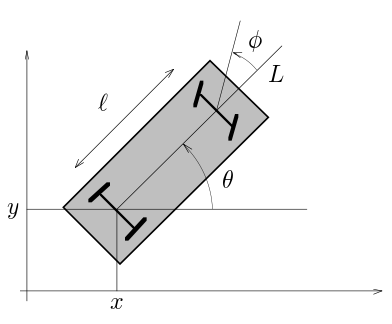
\includegraphics[width=200pt,keepaspectratio=true]{./Vehiculo_traccion_trasera.png}
 % P&ID_anti-suge.png: 0x0 pixel, 300dpi, 0.00x0.00 cm, bb=
  \textit{Figura 1: Diagrama del sistema a estudiar}
\end{center}


\subsection{Se pide}
\begin{enumerate}
\def\labelenumi{\arabic{enumi}.}
\itemsep1pt\parskip0pt\parsep0pt
\item
  Determinar el modelo dinámico del sistema (ecuaciones que permitan
  describir la cinemática del vehículo).

\def\labelenumii{\arabic{enumii}.}
\setcounter{enumii}{1}
\itemsep1pt\parskip0pt\parsep0pt
\item
    Diseñar un algoritmo que permita describir el sistema en el tiempo
    partir de las variables de control \(v(t)\) y \(\psi(t)\).


\def\labelenumiii{\arabic{enumiii}.}
\setcounter{enumiii}{2}
\itemsep1pt\parskip0pt\parsep0pt
\item
      Realizar la representación para varias funciones \(v(t)\) y
      \(\psi(t)\).

\end{enumerate}

\subsection{Solución}
Para determinar el modelo dinámico del sistema se
considerará que las ruedas de la izquierda y las de la derecha son una
sola en el punto medio entre las mismas. Obteniendo de esta manera un
vehículo con dos ruedas, una delantera y una trasera (modelo Half-Car).
La rueda frontal puede rotar un ángulo \(\psi\) al rededor del eje \(z\) y la trasera
esta fija al armazón del vehículo. La rueda delantera gira libremente y
la trasera es la responsable de suministrar la velocidad \(v\). El
vector que determina las corrdenadas del sistema es
\(q = (x, y, \theta, \psi)\) donde \(x\) y \(y\) son las coordenadas en
el plano \(xy\) del punto medio entre las ruedas traseras, \(\theta\) es
el angulo instantáneo de la velocidad con repecto al eje \(x\)
(recordando que la velocidad es tangente a la trayectoria) y \(\psi\) es
el ángulo que giran las ruedas con respecto al vehículo. El sistema
posee dos restricciones no-holónomas, una por cada rueda. \\
\begin{equation}
\label{ec_1}
\begin{array}{lcl} \dot{x}_{f} \sin{\left (\psi + \theta \right )} - \dot{y}_{f} \cos{\left (\psi + \theta \right )} = 0 \\ 
\dot{x} \sin{\left (\theta \right )} - \dot{y} \cos{\left (\theta \right )} = 0 \end{array}
\end{equation} 

Donde \(x_f\) y \(y_f\) representan las coordenadas del punto medio
delantero. Suponiendo que el vehículo es un cuerpo rígido 
\begin{equation}
\label{ec_3}
 x_{f} = l \cos{\left (\theta \right )} + x
\end{equation} 
\begin{equation}
\label{ec_4}
 y_{f} = l \sin{\left (\theta \right )} + y
\end{equation} 

Sustituyendo las ecuaciones (\ref{ec_3}) y (\ref{ec_4}) en (\ref{ec_1}) obtenemos las ecuaciones del sistema
\begin{equation}
\label{ec_5}
\begin{array}{lcl} \dot{\theta} l \cos{\left (\psi \right )} + \dot{x} \sin{\left (\psi + \theta \right )} - \dot{y} \cos{\left (\psi + \theta \right )} = 0 \\ 
\dot{x} \sin{\left (\theta \right )} - \dot{y} \cos{\left (\theta \right )} = 0 \end{array}
\end{equation}


La matriz de restricción del sistema será 

\begin{equation}\adjustbox{max width=\hsize}{$
   \left[\begin{matrix}\sin{\left (\psi + \theta \right )} & \sin{\left (\theta \right )}\\- \cos{\left (\psi + \theta \right )} & - \cos{\left (\theta \right )}\\- l \cos{\left (\theta \right )} & 0\\0 & 0\end{matrix}\right]
$}\end{equation}

 Las velocidades generalizadas del sistema son
 \begin{equation}\adjustbox{max width=\hsize}{$
  \left[\begin{matrix}\dot{x}\\\dot{y}\\\dot{\theta}\\\dot{\psi}\end{matrix}\right] = \left[\begin{matrix}\cos{\left (\psi \right )} \cos{\left (\theta \right )}\\\sin{\left (\theta \right )} \cos{\left (\psi \right )}\\\frac{1}{l} \sin{\left (\psi \right )}\\0\end{matrix}\right]\alpha_1 + \left[\begin{matrix}0\\0\\0\\1\end{matrix}\right] \alpha_2
 $}\end{equation} 

El parámetro $\alpha_2$ corresponde a la razón de cambio del ángulo $\psi$ respecto al tiempo que denomimaremos $u_2$ y $\alpha_1$, al tratarse de un
vehículo de tracción trasera tenemos que sustituirlo por ${u_1} \over {\cos{(\psi)}}$ quedando entonces $u_1=v$. De esta forma las velocidades del sistema serán

 \begin{equation}\adjustbox{max width=\hsize}{$
  \left[\begin{matrix}\dot{x}\\\dot{y}\\\dot{\theta}\\\dot{\psi}\end{matrix}\right] = \left[\begin{matrix}\cos{\left (\theta \right )}\\\sin{\left (\theta \right )} \\\frac{1}{l} \tan{\left (\psi \right )}\\0\end{matrix}\right]u_1 + \left[\begin{matrix}0\\0\\0\\1\end{matrix}\right] u_2
 $}\end{equation} 

El sistema presenta una singularidad cuando la variable de cotrol $\psi$ es igual a $\pi \over 2$.
\end{multicols}

\subsection{Código en python}
El siguiente código escrio en python permite realizar los graficos de posición $xy$, $v(t)$, $\theta(t)$, $\psi(t)$, $x(t)$ y $y(t)$ introduciendo
los valores de $a_0$, $a_1$, $a_2$ y $a_3$ correspondientes al polinomio de grado 3 de la velocidad $v(t) = a_0 + a_1 t + a_2 t^2 + a_3 t^3$, los
valores de $b_0$, $b_1$, $b_2$, $b_3$ correspondientes al polinomio de grado 3 del ángulo $\psi(t) = b_0 + b_1 t + b_2 t^2 + b_3 t^3$ y los valores $x_0$,$y_0$
 y $\theta_0$ correspondientes a los valores de posición inicial del vehículo.


    \begin{Verbatim}[commandchars=\\\{\}]
{\color{incolor}In [{\color{incolor}1}]:} \PY{k+kn}{import} \PY{n+nn}{numpy} \PY{k+kn}{as} \PY{n+nn}{np} \PY{c}{\PYZsh{} Importamos la libreria numerica de python}
        \PY{k+kn}{import} \PY{n+nn}{matplotlib.pyplot} \PY{k+kn}{as} \PY{n+nn}{plt} \PY{c}{\PYZsh{} Importamos la libreria para realizar grficos}
        \PY{k+kn}{from} \PY{n+nn}{\PYZus{}\PYZus{}future\PYZus{}\PYZus{}} \PY{k+kn}{import} \PY{n}{division}
        \PY{o}{\PYZpc{}}\PY{k}{matplotlib} nbagg
        \PY{n}{plt}\PY{o}{.}\PY{n}{style}\PY{o}{.}\PY{n}{use}\PY{p}{(}\PY{l+s}{\PYZsq{}}\PY{l+s}{ggplot}\PY{l+s}{\PYZsq{}}\PY{p}{)} \PY{c}{\PYZsh{} Se usa el estilo ggplot}
        \PY{n}{t\PYZus{}i} \PY{o}{=} \PY{l+m+mi}{0} \PY{c}{\PYZsh{} Tiempo inicial [s]}
        \PY{n}{t\PYZus{}f} \PY{o}{=} \PY{l+m+mi}{5} \PY{c}{\PYZsh{} Tiempo final [s]}
        \PY{n}{n} \PY{o}{=} \PY{l+m+mi}{10000} \PY{c}{\PYZsh{} Numero de iteraciones}
        \PY{n}{t} \PY{o}{=} \PY{n}{np}\PY{o}{.}\PY{n}{linspace}\PY{p}{(}\PY{n}{t\PYZus{}i}\PY{p}{,} \PY{n}{t\PYZus{}f}\PY{p}{,} \PY{n}{n}\PY{p}{)} \PY{c}{\PYZsh{} Se crea el vector t}
        \PY{n}{dt} \PY{o}{=} \PY{p}{(}\PY{n}{t\PYZus{}f} \PY{o}{\PYZhy{}} \PY{n}{t\PYZus{}i}\PY{p}{)} \PY{o}{/} \PY{n}{n} \PY{c}{\PYZsh{} El diferencial de tiempo}
        \PY{n}{l} \PY{o}{=} \PY{l+m+mi}{2} \PY{c}{\PYZsh{} La longitud l}
        \PY{n}{fact} \PY{o}{=} \PY{n}{np}\PY{o}{.}\PY{n}{pi} \PY{o}{/} \PY{l+m+mi}{180} \PY{c}{\PYZsh{} Factor de conversion}
        \PY{k}{def} \PY{n+nf}{posicion}\PY{p}{(}\PY{n}{v}\PY{p}{,}\PY{n}{psi}\PY{p}{,} \PY{n}{theta\PYZus{}i}\PY{p}{,} \PY{n}{x\PYZus{}i}\PY{p}{,}\PY{n}{y\PYZus{}i}\PY{p}{)}\PY{p}{:} \PY{c}{\PYZsh{} Funcion que grafica el comportamiento del vehiculo}
            \PY{n}{theta} \PY{o}{=} \PY{n}{np}\PY{o}{.}\PY{n}{zeros}\PY{p}{(}\PY{n}{n}\PY{p}{)}
            \PY{n}{theta}\PY{p}{[}\PY{l+m+mi}{0}\PY{p}{]} \PY{o}{=} \PY{n}{theta\PYZus{}i}
            \PY{n}{x} \PY{o}{=} \PY{n}{np}\PY{o}{.}\PY{n}{zeros}\PY{p}{(}\PY{n}{n}\PY{p}{)}
            \PY{n}{y} \PY{o}{=} \PY{n}{np}\PY{o}{.}\PY{n}{zeros}\PY{p}{(}\PY{n}{n}\PY{p}{)}
            \PY{n}{x}\PY{p}{[}\PY{l+m+mi}{0}\PY{p}{]} \PY{o}{=} \PY{n}{x\PYZus{}i}
            \PY{n}{y}\PY{p}{[}\PY{l+m+mi}{0}\PY{p}{]} \PY{o}{=} \PY{n}{y\PYZus{}i}
            \PY{k}{for} \PY{n}{i} \PY{o+ow}{in} \PY{n+nb}{range}\PY{p}{(}\PY{n}{n}\PY{o}{\PYZhy{}}\PY{l+m+mi}{1}\PY{p}{)}\PY{p}{:}
                \PY{k}{if}\PY{p}{(}\PY{n}{psi}\PY{p}{[}\PY{n}{i}\PY{p}{]}\PY{o}{\PYZgt{}}\PY{n}{np}\PY{o}{.}\PY{n}{pi}\PY{o}{/}\PY{l+m+mi}{2}\PY{o}{\PYZhy{}}\PY{l+m+mf}{0.001}\PY{p}{)}\PY{p}{:}
                    \PY{n}{psi}\PY{p}{[}\PY{n}{i}\PY{p}{]} \PY{o}{=} \PY{n}{np}\PY{o}{.}\PY{n}{pi} \PY{o}{/} \PY{l+m+mi}{2} \PY{o}{\PYZhy{}} \PY{l+m+mf}{0.001}
                \PY{k}{if} \PY{n}{psi}\PY{p}{[}\PY{n}{i}\PY{p}{]}\PY{o}{\PYZlt{}}\PY{o}{\PYZhy{}}\PY{n}{np}\PY{o}{.}\PY{n}{pi}\PY{o}{/}\PY{l+m+mi}{2}\PY{o}{+}\PY{l+m+mf}{0.001}\PY{p}{:}
                    \PY{n}{psi}\PY{p}{[}\PY{n}{i}\PY{p}{]} \PY{o}{=} \PY{o}{\PYZhy{}}\PY{n}{np}\PY{o}{.}\PY{n}{pi} \PY{o}{/} \PY{l+m+mi}{2} \PY{o}{+} \PY{l+m+mf}{0.001}
                \PY{n}{theta}\PY{p}{[}\PY{n}{i}\PY{o}{+}\PY{l+m+mi}{1}\PY{p}{]} \PY{o}{=} \PY{n}{theta}\PY{p}{[}\PY{n}{i}\PY{p}{]} \PY{o}{+} \PY{p}{(}\PY{n}{v}\PY{p}{[}\PY{n}{i}\PY{p}{]} \PY{o}{/} \PY{n}{l}\PY{p}{)}\PY{o}{*}\PY{n}{np}\PY{o}{.}\PY{n}{tan}\PY{p}{(}\PY{n}{psi}\PY{p}{[}\PY{n}{i}\PY{o}{+}\PY{l+m+mi}{1}\PY{p}{]}\PY{p}{)} \PY{o}{*} \PY{n}{dt}
                \PY{n}{x}\PY{p}{[}\PY{n}{i}\PY{o}{+}\PY{l+m+mi}{1}\PY{p}{]} \PY{o}{=} \PY{n}{x}\PY{p}{[}\PY{n}{i}\PY{p}{]} \PY{o}{+} \PY{n}{v}\PY{p}{[}\PY{n}{i}\PY{p}{]} \PY{o}{*} \PY{n}{np}\PY{o}{.}\PY{n}{cos}\PY{p}{(}\PY{n}{theta}\PY{p}{[}\PY{n}{i}\PY{p}{]}\PY{p}{)} \PY{o}{*} \PY{n}{dt}
                \PY{n}{y}\PY{p}{[}\PY{n}{i}\PY{o}{+}\PY{l+m+mi}{1}\PY{p}{]} \PY{o}{=} \PY{n}{y}\PY{p}{[}\PY{n}{i}\PY{p}{]} \PY{o}{+} \PY{n}{v}\PY{p}{[}\PY{n}{i}\PY{p}{]} \PY{o}{*} \PY{n}{np}\PY{o}{.}\PY{n}{sin}\PY{p}{(}\PY{n}{theta}\PY{p}{[}\PY{n}{i}\PY{p}{]}\PY{p}{)} \PY{o}{*} \PY{n}{dt}
            \PY{n}{grafico} \PY{o}{=} \PY{n}{plt}\PY{o}{.}\PY{n}{figure}\PY{p}{(}\PY{p}{)}
            \PY{n}{pos\PYZus{}plt} \PY{o}{=} \PY{n}{grafico}\PY{o}{.}\PY{n}{add\PYZus{}subplot}\PY{p}{(}\PY{l+m+mi}{321}\PY{p}{)}
            \PY{n}{pos\PYZus{}plt}\PY{o}{.}\PY{n}{plot}\PY{p}{(}\PY{n}{x}\PY{p}{,}\PY{n}{y}\PY{p}{)}
            \PY{n}{pos\PYZus{}plt}\PY{o}{.}\PY{n}{set\PYZus{}title}\PY{p}{(}\PY{l+s}{\PYZsq{}}\PY{l+s}{Posicion del vehiculo}\PY{l+s}{\PYZsq{}}\PY{p}{)}
            \PY{n}{vel\PYZus{}plt} \PY{o}{=} \PY{n}{grafico}\PY{o}{.}\PY{n}{add\PYZus{}subplot}\PY{p}{(}\PY{l+m+mi}{322}\PY{p}{)}
            \PY{n}{vel\PYZus{}plt}\PY{o}{.}\PY{n}{plot}\PY{p}{(}\PY{n}{t}\PY{p}{,}\PY{n}{v}\PY{p}{)}
            \PY{n}{vel\PYZus{}plt}\PY{o}{.}\PY{n}{set\PYZus{}title}\PY{p}{(}\PY{l+s}{\PYZsq{}}\PY{l+s}{Velocidad del vehiculo}\PY{l+s}{\PYZsq{}}\PY{p}{)}
            \PY{n}{theta\PYZus{}plt} \PY{o}{=} \PY{n}{grafico}\PY{o}{.}\PY{n}{add\PYZus{}subplot}\PY{p}{(}\PY{l+m+mi}{323}\PY{p}{)}
            \PY{n}{theta\PYZus{}plt}\PY{o}{.}\PY{n}{plot}\PY{p}{(}\PY{n}{t}\PY{p}{,}\PY{n}{theta}\PY{p}{)}
            \PY{n}{theta\PYZus{}plt}\PY{o}{.}\PY{n}{set\PYZus{}title}\PY{p}{(}\PY{l+s}{\PYZsq{}}\PY{l+s}{Angulo theta}\PY{l+s}{\PYZsq{}}\PY{p}{)}
            \PY{n}{psi\PYZus{}plt} \PY{o}{=} \PY{n}{grafico}\PY{o}{.}\PY{n}{add\PYZus{}subplot}\PY{p}{(}\PY{l+m+mi}{324}\PY{p}{)}
            \PY{n}{psi\PYZus{}plt}\PY{o}{.}\PY{n}{plot}\PY{p}{(}\PY{n}{t}\PY{p}{,}\PY{n}{psi}\PY{p}{)}
            \PY{n}{psi\PYZus{}plt}\PY{o}{.}\PY{n}{set\PYZus{}title}\PY{p}{(}\PY{l+s}{\PYZsq{}}\PY{l+s}{Angulo psi}\PY{l+s}{\PYZsq{}}\PY{p}{)}
            \PY{n}{x\PYZus{}plt} \PY{o}{=} \PY{n}{grafico}\PY{o}{.}\PY{n}{add\PYZus{}subplot}\PY{p}{(}\PY{l+m+mi}{325}\PY{p}{)}
            \PY{n}{x\PYZus{}plt}\PY{o}{.}\PY{n}{plot}\PY{p}{(}\PY{n}{t}\PY{p}{,}\PY{n}{x}\PY{p}{)}
            \PY{n}{x\PYZus{}plt}\PY{o}{.}\PY{n}{set\PYZus{}title}\PY{p}{(}\PY{l+s}{\PYZsq{}}\PY{l+s}{x(t)}\PY{l+s}{\PYZsq{}}\PY{p}{)}
            \PY{n}{y\PYZus{}plt} \PY{o}{=} \PY{n}{grafico}\PY{o}{.}\PY{n}{add\PYZus{}subplot}\PY{p}{(}\PY{l+m+mi}{326}\PY{p}{)}
            \PY{n}{y\PYZus{}plt}\PY{o}{.}\PY{n}{plot}\PY{p}{(}\PY{n}{t}\PY{p}{,}\PY{n}{y}\PY{p}{)}
            \PY{n}{y\PYZus{}plt}\PY{o}{.}\PY{n}{set\PYZus{}title}\PY{p}{(}\PY{l+s}{\PYZsq{}}\PY{l+s}{y(t)}\PY{l+s}{\PYZsq{}}\PY{p}{)}
            \PY{n}{grafico}\PY{o}{.}\PY{n}{show}\PY{p}{(}\PY{p}{)}
\end{Verbatim}

    \begin{Verbatim}[commandchars=\\\{\}]
{\color{incolor}In [{\color{incolor}2}]:} \PY{k+kn}{from} \PY{n+nn}{IPython.html.widgets} \PY{k+kn}{import} \PY{n}{interact}\PY{p}{,} \PY{n}{FloatSlider}\PY{p}{,} \PY{n}{interactive}
        \PY{k+kn}{from} \PY{n+nn}{IPython.display} \PY{k+kn}{import} \PY{n}{display}
        \PY{k}{def} \PY{n+nf}{graficar}\PY{p}{(}\PY{n}{a\PYZus{}0}\PY{p}{,}\PY{n}{a\PYZus{}1}\PY{p}{,}\PY{n}{a\PYZus{}2}\PY{p}{,}\PY{n}{a\PYZus{}3}\PY{p}{,}\PY{n}{b\PYZus{}0}\PY{p}{,}\PY{n}{b\PYZus{}1}\PY{p}{,}\PY{n}{b\PYZus{}2}\PY{p}{,}\PY{n}{b\PYZus{}3}\PY{p}{,}\PY{n}{x\PYZus{}0}\PY{p}{,}\PY{n}{y\PYZus{}0}\PY{p}{,}\PY{n}{theta\PYZus{}0}\PY{p}{)}\PY{p}{:}
            \PY{n}{v} \PY{o}{=} \PY{n}{np}\PY{o}{.}\PY{n}{zeros}\PY{p}{(}\PY{n}{n}\PY{p}{)}
            \PY{n}{psi} \PY{o}{=} \PY{n}{np}\PY{o}{.}\PY{n}{zeros}\PY{p}{(}\PY{n}{n}\PY{p}{)}
            \PY{n}{v} \PY{o}{=} \PY{n}{a\PYZus{}0} \PY{o}{+} \PY{n}{a\PYZus{}1} \PY{o}{*} \PY{n}{t} \PY{o}{+} \PY{n}{a\PYZus{}2} \PY{o}{*} \PY{n}{t}\PY{o}{*}\PY{o}{*}\PY{l+m+mi}{2} \PY{o}{+} \PY{n}{a\PYZus{}3} \PY{o}{*} \PY{n}{t}\PY{o}{*}\PY{o}{*}\PY{l+m+mi}{3}
            \PY{n}{psi} \PY{o}{=} \PY{p}{(}\PY{n}{b\PYZus{}0} \PY{o}{+} \PY{n}{b\PYZus{}1} \PY{o}{*} \PY{n}{t} \PY{o}{+} \PY{n}{b\PYZus{}2} \PY{o}{*} \PY{n}{t}\PY{o}{*}\PY{o}{*}\PY{l+m+mi}{2} \PY{o}{+} \PY{n}{b\PYZus{}3} \PY{o}{*} \PY{n}{t}\PY{o}{*}\PY{o}{*}\PY{l+m+mi}{3}\PY{p}{)}
            \PY{n}{posicion}\PY{p}{(}\PY{n}{v}\PY{p}{,}\PY{n}{psi}\PY{p}{,}\PY{n}{theta\PYZus{}0}\PY{p}{,}\PY{n}{x\PYZus{}0}\PY{p}{,}\PY{n}{y\PYZus{}0}\PY{p}{)}
        \PY{n}{a\PYZus{}0\PYZus{}slider} \PY{o}{=} \PY{n}{FloatSlider}\PY{p}{(}\PY{n+nb}{min}\PY{o}{=}\PY{o}{\PYZhy{}}\PY{l+m+mi}{10}\PY{p}{,} \PY{n+nb}{max}\PY{o}{=}\PY{l+m+mi}{10}\PY{p}{,} \PY{n}{step}\PY{o}{=}\PY{l+m+mf}{0.1}\PY{p}{,} \PY{n}{value}\PY{o}{=}\PY{l+m+mi}{5}\PY{p}{,} \PY{n}{description}\PY{o}{=}\PY{l+s}{\PYZsq{}}\PY{l+s}{\PYZdl{}a\PYZus{}0\PYZdl{}}\PY{l+s}{\PYZsq{}}\PY{p}{)}
        \PY{n}{a\PYZus{}1\PYZus{}slider} \PY{o}{=} \PY{n}{FloatSlider}\PY{p}{(}\PY{n+nb}{min}\PY{o}{=}\PY{o}{\PYZhy{}}\PY{l+m+mi}{4}\PY{p}{,} \PY{n+nb}{max}\PY{o}{=}\PY{l+m+mi}{4}\PY{p}{,} \PY{n}{step}\PY{o}{=}\PY{l+m+mf}{0.1}\PY{p}{,} \PY{n}{value}\PY{o}{=}\PY{l+m+mi}{1}\PY{p}{,} \PY{n}{description}\PY{o}{=}\PY{l+s}{\PYZsq{}}\PY{l+s}{\PYZdl{}a\PYZus{}1\PYZdl{}}\PY{l+s}{\PYZsq{}}\PY{p}{)}
        \PY{n}{a\PYZus{}2\PYZus{}slider} \PY{o}{=} \PY{n}{FloatSlider}\PY{p}{(}\PY{n+nb}{min}\PY{o}{=}\PY{o}{\PYZhy{}}\PY{l+m+mi}{1}\PY{p}{,} \PY{n+nb}{max}\PY{o}{=}\PY{l+m+mi}{1}\PY{p}{,} \PY{n}{step}\PY{o}{=}\PY{l+m+mf}{0.1}\PY{p}{,} \PY{n}{value}\PY{o}{=}\PY{l+m+mi}{0}\PY{p}{,} \PY{n}{description}\PY{o}{=}\PY{l+s}{\PYZsq{}}\PY{l+s}{\PYZdl{}a\PYZus{}2\PYZdl{}}\PY{l+s}{\PYZsq{}}\PY{p}{)}
        \PY{n}{a\PYZus{}3\PYZus{}slider} \PY{o}{=} \PY{n}{FloatSlider}\PY{p}{(}\PY{n+nb}{min}\PY{o}{=}\PY{o}{\PYZhy{}}\PY{l+m+mi}{1}\PY{p}{,} \PY{n+nb}{max}\PY{o}{=}\PY{l+m+mi}{1}\PY{p}{,} \PY{n}{step}\PY{o}{=}\PY{l+m+mf}{0.1}\PY{p}{,} \PY{n}{value}\PY{o}{=}\PY{l+m+mi}{0}\PY{p}{,} \PY{n}{description}\PY{o}{=}\PY{l+s}{\PYZsq{}}\PY{l+s}{\PYZdl{}a\PYZus{}3\PYZdl{}}\PY{l+s}{\PYZsq{}}\PY{p}{)}
        \PY{n}{b\PYZus{}0\PYZus{}slider} \PY{o}{=} \PY{n}{FloatSlider}\PY{p}{(}\PY{n+nb}{min}\PY{o}{=}\PY{o}{\PYZhy{}}\PY{n}{np}\PY{o}{.}\PY{n}{pi}\PY{o}{/}\PY{l+m+mi}{2}\PY{p}{,} \PY{n+nb}{max}\PY{o}{=}\PY{n}{np}\PY{o}{.}\PY{n}{pi}\PY{o}{/}\PY{l+m+mi}{2}\PY{p}{,} \PY{n}{step}\PY{o}{=}\PY{l+m+mf}{0.05}\PY{p}{,} \PY{n}{value}\PY{o}{=}\PY{n}{np}\PY{o}{.}\PY{n}{pi}\PY{o}{/}\PY{l+m+mi}{4}\PY{p}{,} \PY{n}{description}\PY{o}{=}\PY{l+s}{\PYZsq{}}\PY{l+s}{\PYZdl{}b\PYZus{}0\PYZdl{}}\PY{l+s}{\PYZsq{}}\PY{p}{)}
        \PY{n}{b\PYZus{}1\PYZus{}slider} \PY{o}{=} \PY{n}{FloatSlider}\PY{p}{(}\PY{n+nb}{min}\PY{o}{=}\PY{o}{\PYZhy{}}\PY{n}{np}\PY{o}{.}\PY{n}{pi}\PY{o}{/}\PY{l+m+mi}{2}\PY{p}{,} \PY{n+nb}{max}\PY{o}{=}\PY{n}{np}\PY{o}{.}\PY{n}{pi}\PY{o}{/}\PY{l+m+mi}{2}\PY{p}{,} \PY{n}{step}\PY{o}{=}\PY{l+m+mf}{0.05}\PY{p}{,} \PY{n}{value}\PY{o}{=}\PY{l+m+mi}{0}\PY{p}{,} \PY{n}{description}\PY{o}{=}\PY{l+s}{\PYZsq{}}\PY{l+s}{\PYZdl{}b\PYZus{}1\PYZdl{}}\PY{l+s}{\PYZsq{}}\PY{p}{)}
        \PY{n}{b\PYZus{}2\PYZus{}slider} \PY{o}{=} \PY{n}{FloatSlider}\PY{p}{(}\PY{n+nb}{min}\PY{o}{=}\PY{o}{\PYZhy{}}\PY{l+m+mi}{1}\PY{p}{,} \PY{n+nb}{max}\PY{o}{=}\PY{l+m+mi}{1}\PY{p}{,} \PY{n}{step}\PY{o}{=}\PY{l+m+mf}{0.1}\PY{p}{,} \PY{n}{value}\PY{o}{=}\PY{l+m+mi}{0}\PY{p}{,} \PY{n}{description}\PY{o}{=}\PY{l+s}{\PYZsq{}}\PY{l+s}{\PYZdl{}b\PYZus{}2\PYZdl{}}\PY{l+s}{\PYZsq{}}\PY{p}{)}
        \PY{n}{b\PYZus{}3\PYZus{}slider} \PY{o}{=} \PY{n}{FloatSlider}\PY{p}{(}\PY{n+nb}{min}\PY{o}{=}\PY{o}{\PYZhy{}}\PY{l+m+mi}{1}\PY{p}{,} \PY{n+nb}{max}\PY{o}{=}\PY{l+m+mi}{1}\PY{p}{,} \PY{n}{step}\PY{o}{=}\PY{l+m+mf}{0.1}\PY{p}{,} \PY{n}{value}\PY{o}{=}\PY{l+m+mi}{0}\PY{p}{,} \PY{n}{description}\PY{o}{=}\PY{l+s}{\PYZsq{}}\PY{l+s}{\PYZdl{}b\PYZus{}3\PYZdl{}}\PY{l+s}{\PYZsq{}}\PY{p}{)}
        \PY{n}{x\PYZus{}0\PYZus{}slider} \PY{o}{=} \PY{n}{FloatSlider}\PY{p}{(}\PY{n+nb}{min}\PY{o}{=}\PY{o}{\PYZhy{}}\PY{l+m+mi}{10}\PY{p}{,} \PY{n+nb}{max}\PY{o}{=}\PY{l+m+mi}{10}\PY{p}{,} \PY{n}{step}\PY{o}{=}\PY{l+m+mf}{0.1}\PY{p}{,} \PY{n}{value}\PY{o}{=}\PY{l+m+mi}{0}\PY{p}{,} \PY{n}{description}\PY{o}{=}\PY{l+s}{\PYZsq{}}\PY{l+s}{\PYZdl{}x\PYZus{}0\PYZdl{}}\PY{l+s}{\PYZsq{}}\PY{p}{)}
        \PY{n}{y\PYZus{}0\PYZus{}slider} \PY{o}{=} \PY{n}{FloatSlider}\PY{p}{(}\PY{n+nb}{min}\PY{o}{=}\PY{o}{\PYZhy{}}\PY{l+m+mi}{10}\PY{p}{,} \PY{n+nb}{max}\PY{o}{=}\PY{l+m+mi}{10}\PY{p}{,} \PY{n}{step}\PY{o}{=}\PY{l+m+mf}{0.1}\PY{p}{,} \PY{n}{value}\PY{o}{=}\PY{l+m+mi}{0}\PY{p}{,} \PY{n}{description}\PY{o}{=}\PY{l+s}{\PYZsq{}}\PY{l+s}{\PYZdl{}y\PYZus{}0\PYZdl{}}\PY{l+s}{\PYZsq{}}\PY{p}{)}
        \PY{n}{theta\PYZus{}0\PYZus{}slider} \PY{o}{=} \PY{n}{FloatSlider}\PY{p}{(}\PY{n+nb}{min}\PY{o}{=}\PY{o}{\PYZhy{}}\PY{l+m+mi}{2}\PY{o}{*}\PY{n}{np}\PY{o}{.}\PY{n}{pi}\PY{p}{,} \PY{n+nb}{max}\PY{o}{=}\PY{l+m+mi}{2}\PY{o}{*}\PY{n}{np}\PY{o}{.}\PY{n}{pi}\PY{p}{,} \PY{n}{step}\PY{o}{=}\PY{l+m+mf}{0.1}\PY{p}{,} \PY{n}{value}\PY{o}{=}\PY{l+m+mi}{0}\PY{p}{,}
                                     \PY{n}{description}\PY{o}{=}\PY{l+s}{\PYZsq{}}\PY{l+s}{\PYZdl{}}\PY{l+s+se}{\PYZbs{}\PYZbs{}}\PY{l+s}{theta\PYZus{}0\PYZdl{}}\PY{l+s}{\PYZsq{}}\PY{p}{)}
        \PY{n}{w}\PY{o}{=}\PY{n}{interactive}\PY{p}{(}\PY{n}{graficar}\PY{p}{,}\PY{n}{a\PYZus{}0}\PY{o}{=}\PY{n}{a\PYZus{}0\PYZus{}slider}\PY{p}{,}\PY{n}{a\PYZus{}1}\PY{o}{=}\PY{n}{a\PYZus{}1\PYZus{}slider}\PY{p}{,}\PY{n}{a\PYZus{}2}\PY{o}{=}\PY{n}{a\PYZus{}2\PYZus{}slider}\PY{p}{,}\PY{n}{a\PYZus{}3}\PY{o}{=}\PY{n}{a\PYZus{}3\PYZus{}slider}\PY{p}{,}
                      \PY{n}{b\PYZus{}0}\PY{o}{=}\PY{n}{b\PYZus{}0\PYZus{}slider}\PY{p}{,} \PY{n}{b\PYZus{}1}\PY{o}{=}\PY{n}{b\PYZus{}1\PYZus{}slider}\PY{p}{,} \PY{n}{b\PYZus{}2}\PY{o}{=}\PY{n}{b\PYZus{}2\PYZus{}slider}\PY{p}{,} \PY{n}{b\PYZus{}3}\PY{o}{=}\PY{n}{b\PYZus{}3\PYZus{}slider}\PY{p}{,}
                      \PY{n}{x\PYZus{}0}\PY{o}{=}\PY{n}{x\PYZus{}0\PYZus{}slider}\PY{p}{,} \PY{n}{y\PYZus{}0}\PY{o}{=}\PY{n}{y\PYZus{}0\PYZus{}slider}\PY{p}{,} \PY{n}{theta\PYZus{}0}\PY{o}{=}\PY{n}{theta\PYZus{}0\PYZus{}slider}\PY{p}{)}
        \PY{n}{display}\PY{p}{(}\PY{n}{w}\PY{p}{)}
\end{Verbatim}

\begin{multicols}{2}
\subsection{Resultados}
\subsubsection{Velocidad $V(t)$ y Ángulo $\psi(t)$ constantes}
\begin{center}
 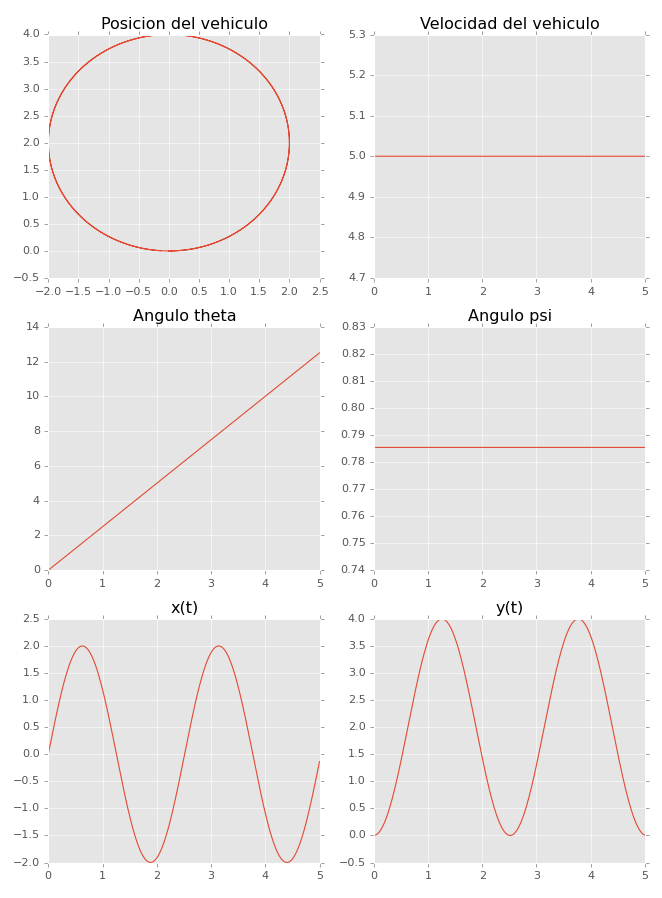
\includegraphics[width=240pt,height=325pt]{./v_const_psi_const.png}
 % P&ID_anti-suge.png: 0x0 pixel, 300dpi, 0.00x0.00 cm, bb=
  \textit{Figura 2: Velocidad $V(t)$ y Ángulo $\psi(t)$ constantes}
\end{center}
\vspace*{7\baselineskip}
\subsubsection{Velocidad $V(t)$ lineal y Ángulo $\psi(t)$ constante}
\begin{center}
 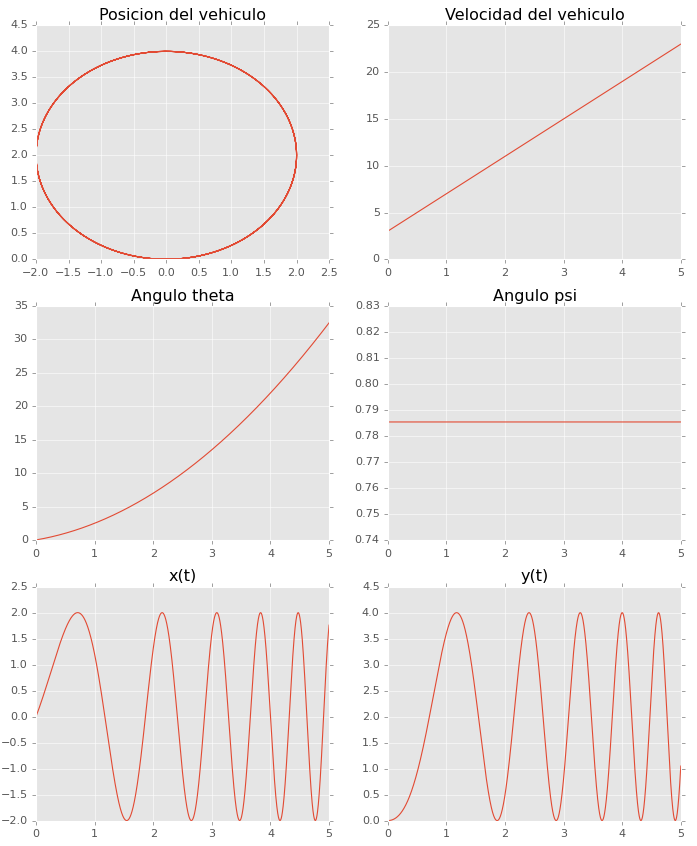
\includegraphics[width=240pt,height=325pt]{./v_lin_psi_const.png}
 % P&ID_anti-suge.png: 0x0 pixel, 300dpi, 0.00x0.00 cm, bb=
  \textit{Figura 3: Velocidad $V(t)$ lineal y Ángulo $\psi(t)$ constante}
\end{center}

\subsubsection{Velocidad $V(t)$ lineal y Ángulo $\psi(t)$ lineal}
\begin{center}
 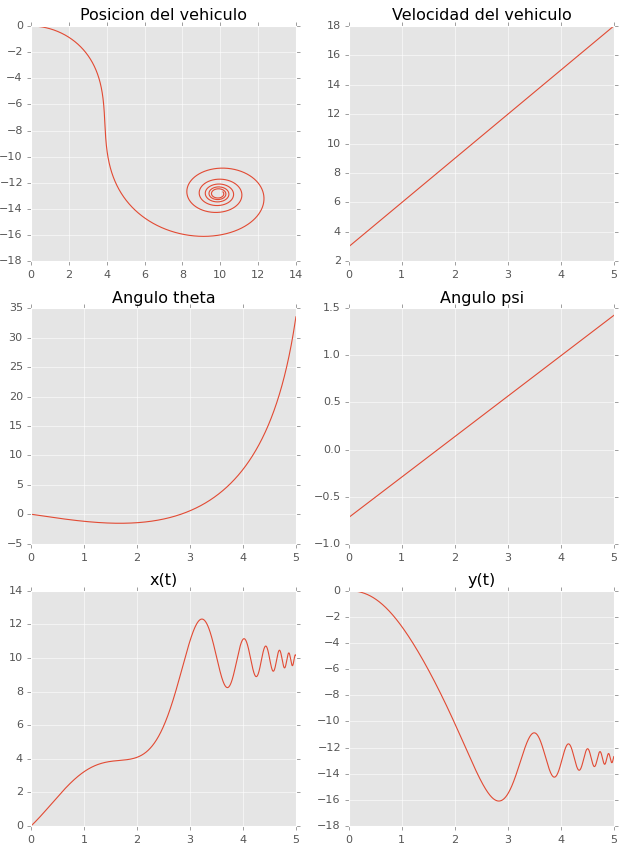
\includegraphics[width=240pt,height=325pt]{./v_lin_psi_lin.png}
 % P&ID_anti-suge.png: 0x0 pixel, 300dpi, 0.00x0.00 cm, bb=
  \textit{Figura 3: Velocidad $V(t)$ lineal y Ángulo $\psi(t)$ lineal}
\end{center}

\subsubsection{Velocidad $V(t)$ cuadrática y Ángulo $\psi(t)$ lineal}
\begin{center}
 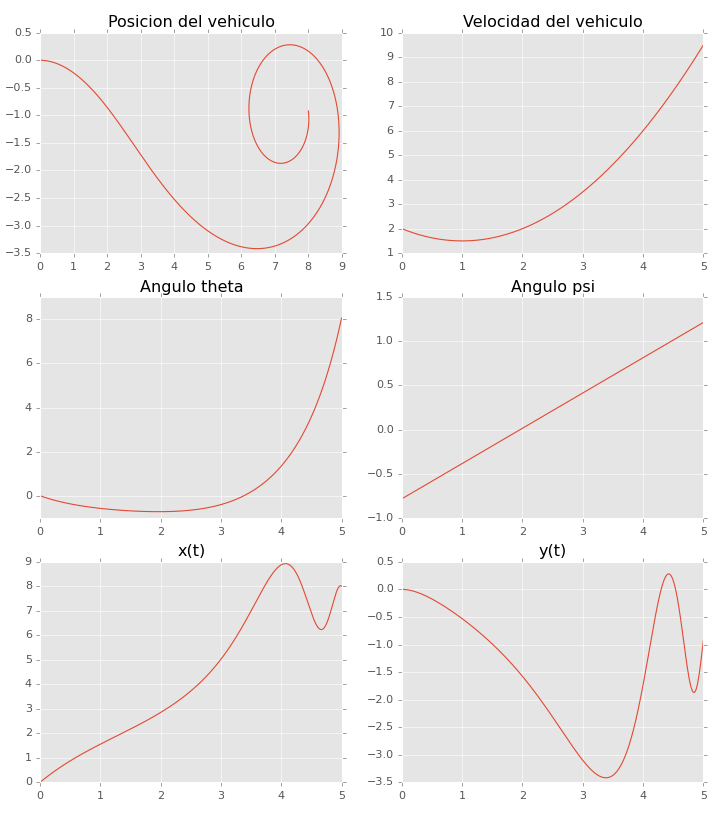
\includegraphics[width=240pt,height=325pt]{./v_quad_psi_lin.png}
 % P&ID_anti-suge.png: 0x0 pixel, 300dpi, 0.00x0.00 cm, bb=
  \textit{Figura 3: Velocidad $V(t)$ cuadrática y Ángulo $\psi(t)$ lineal}
\end{center}

\subsubsection{Velocidad $V(t)$ lineal y Ángulo $\psi(t)$ cuadrática}
\begin{center}
 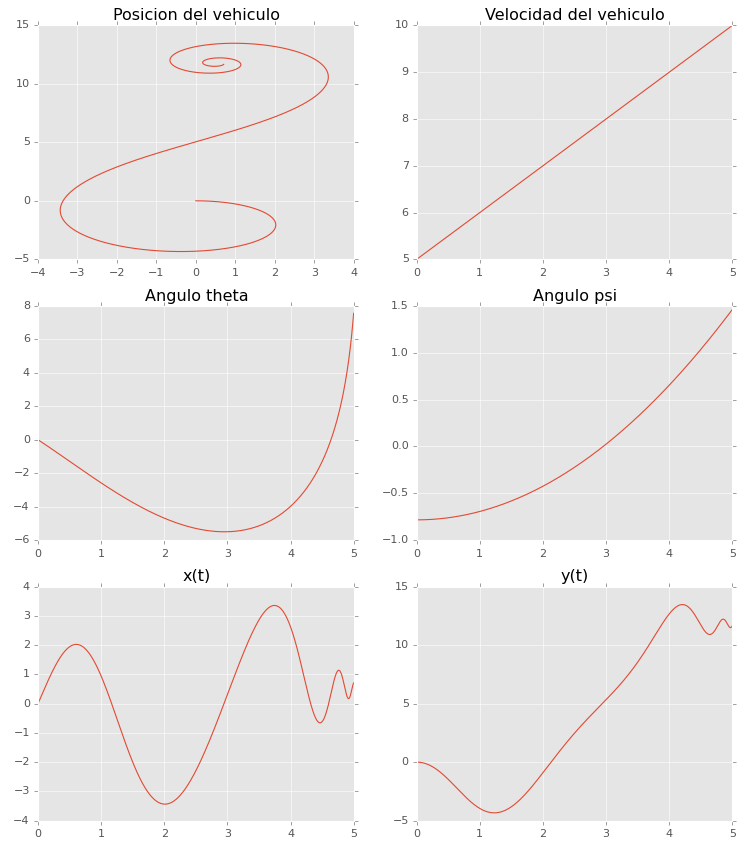
\includegraphics[width=240pt,height=325pt]{./v_lin_psi_quad.png}
 % P&ID_anti-suge.png: 0x0 pixel, 300dpi, 0.00x0.00 cm, bb=
  \textit{Figura 3: Velocidad $V(t)$ lineal y Ángulo $\psi(t)$ cuadrática}
\end{center}

\subsubsection{Velocidad $V(t)$ cuadrática y Ángulo $\psi(t)$ cuadrática}
\begin{center}
 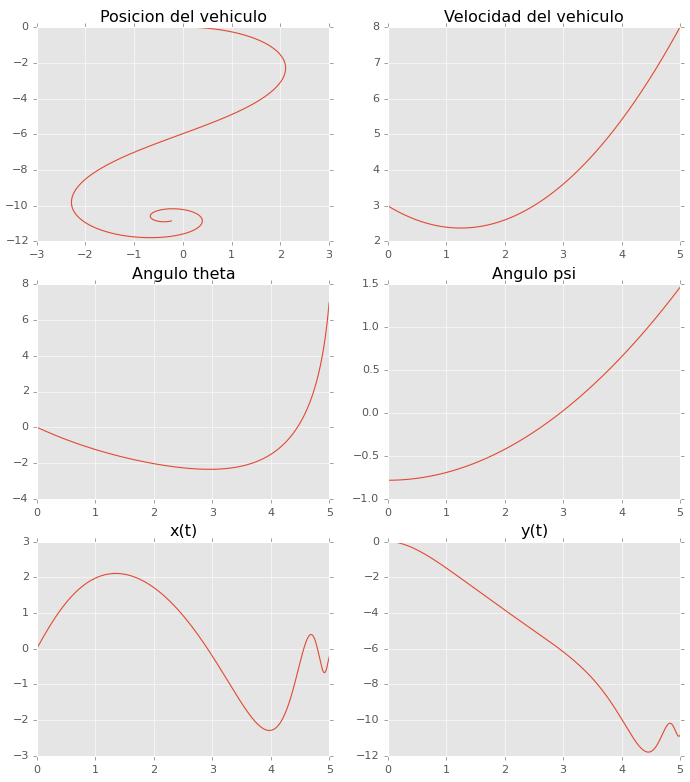
\includegraphics[width=240pt,height=325pt]{./v_quad_psi_quad.png}
 % P&ID_anti-suge.png: 0x0 pixel, 300dpi, 0.00x0.00 cm, bb=
  \textit{Figura 3: Velocidad $V(t)$ cuadrática y Ángulo $\psi(t)$ cuadrática}
\end{center}



\end{multicols}
\end{document}
